本次退款口径下的实际总费用为12,972,155.14元，紧急购电量为38,802.76\,kWh，下调取消电量为649,618.04\,kWh。表\ref{tab:q3-cost}将退款与支出分别列出，全部费用由实际执行轨迹逐槽结算。
\begin{table}[htbp]
\centering\small
\caption{第三问334日实际费用分解}\label{tab:q3-cost}
\begin{tabular}{lr}
\toprule
项目 & 金额/元\\
\midrule
原计划购电费 & 12,163,951.80\\
上调追加费 & 845,883.89\\
下调退款（扣减） & -225,481.41\\
紧急购电费 & 187,800.86\\
总费用 & 12,972,155.14\\
\bottomrule
\end{tabular}
\end{table}
\begin{table}[htbp]
\centering\small
\caption{四个指定日的计划购电与实际总费用}\label{tab:q3-daily}
\begin{tabular}{lrrr}
\toprule
日期 & 原计划/kWh & 最终常规购电/kWh & 实际总费用/元\\
\midrule
03-20 & 63,541.25 & 64,216.25 & 41,895.38\\
06-21 & 29,443.98 & 30,371.48 & 18,014.76\\
09-23 & 67,736.57 & 65,508.65 & 43,855.74\\
12-21 & 91,642.02 & 92,538.94 & 62,181.06\\
\bottomrule
\end{tabular}
\end{table}
\begin{table}[htbp]
\centering\small
\caption{指定十分钟区间的原计划与最终购电量（kWh）}\label{tab:q3-slots}
\begin{tabular}{llrr}
\toprule
日期 & 时段 & 原计划 & 最终购电\\
\midrule
03-20 & 10:00--10:10 & 0.00 & 0.00\\
03-20 & 12:00--12:10 & 644.77 & 639.05\\
03-20 & 14:00--14:10 & 3.37 & 3.37\\
03-20 & 16:00--16:10 & 642.14 & 642.14\\
03-20 & 18:00--18:10 & 684.13 & 696.70\\
03-20 & 20:00--20:10 & 0.00 & 0.00\\
06-21 & 10:00--10:10 & 0.00 & 0.00\\
06-21 & 12:00--12:10 & 0.00 & 0.00\\
06-21 & 14:00--14:10 & 0.00 & 0.00\\
06-21 & 16:00--16:10 & 97.34 & 97.34\\
06-21 & 18:00--18:10 & 114.66 & 136.84\\
06-21 & 20:00--20:10 & 0.00 & 0.00\\
09-23 & 10:00--10:10 & 0.00 & 0.00\\
09-23 & 12:00--12:10 & 419.77 & 91.84\\
09-23 & 14:00--14:10 & 0.00 & 0.00\\
09-23 & 16:00--16:10 & 524.10 & 524.10\\
09-23 & 18:00--18:10 & 725.46 & 782.79\\
09-23 & 20:00--20:10 & 31.91 & 31.91\\
12-21 & 10:00--10:10 & 0.00 & 0.00\\
12-21 & 12:00--12:10 & 1,012.76 & 942.11\\
12-21 & 14:00--14:10 & 0.00 & 0.00\\
12-21 & 16:00--16:10 & 842.47 & 868.04\\
12-21 & 18:00--18:10 & 668.86 & 668.86\\
12-21 & 20:00--20:10 & 0.00 & 0.00\\
\bottomrule
\end{tabular}
\end{table}
\begin{table}[htbp]
\centering\small
\caption{指定日期的四小时充放电量（kWh）}\label{tab:q3-storage}
\begin{tabular}{llrr}
\toprule
日期 & 时段 & 充电量 & 放电量\\
\midrule
03-20 & 0:00--4:00 & 7,633.02 & 113.03\\
03-20 & 4:00--8:00 & 2,110.07 & 6,617.47\\
03-20 & 8:00--12:00 & 3,212.10 & 2,677.32\\
03-20 & 12:00--16:00 & 5,565.02 & 70.77\\
03-20 & 16:00--20:00 & 590.70 & 5,330.44\\
03-20 & 20:00--24:00 & 294.94 & 3,102.66\\
06-21 & 0:00--4:00 & 129.38 & 910.73\\
06-21 & 4:00--8:00 & 1,094.24 & 2,000.69\\
06-21 & 8:00--12:00 & 9,783.17 & 0.00\\
06-21 & 12:00--16:00 & 0.00 & 0.00\\
06-21 & 16:00--20:00 & 0.00 & 6,403.89\\
06-21 & 20:00--24:00 & 1,029.25 & 2,748.06\\
09-23 & 0:00--4:00 & 7,583.79 & 97.29\\
09-23 & 4:00--8:00 & 1,412.59 & 6,117.09\\
09-23 & 8:00--12:00 & 5,038.21 & 1,896.62\\
09-23 & 12:00--16:00 & 4,622.62 & 343.55\\
09-23 & 16:00--20:00 & 0.00 & 5,895.68\\
09-23 & 20:00--24:00 & 1,339.09 & 3,257.86\\
12-21 & 0:00--4:00 & 8,799.86 & 124.90\\
12-21 & 4:00--8:00 & 3,153.28 & 2,578.27\\
12-21 & 8:00--12:00 & 5,074.62 & 8,062.09\\
12-21 & 12:00--16:00 & 7,985.19 & 2,646.47\\
12-21 & 16:00--20:00 & 0.00 & 6,478.29\\
12-21 & 20:00--24:00 & 345.74 & 2,759.01\\
\bottomrule
\end{tabular}
\end{table}
\begin{table}[htbp]
\centering\small
\caption{指定日期的日初与日末储电量}\label{tab:q3-soc}
\begin{tabular}{lrr}
\toprule
日期 & 0:00储电量/kWh & 24:00储电量/kWh\\
\midrule
03-20 & 1,873.61 & 1,403.03\\
06-21 & 3,426.95 & 2,129.43\\
09-23 & 1,918.51 & 2,328.09\\
12-21 & 1,207.83 & 1,391.03\\
\bottomrule
\end{tabular}
\end{table}
\begin{table}[htbp]
\centering\small
\caption{指定日期的完整紧急购电区间}\label{tab:q3-emergency}
\begin{tabular}{llr}
\toprule
日期 & 时间段 & 紧急购电量/kWh\\
\midrule
03-20 & 09:30--10:00 & 100.06\\
06-21 & 06:30--07:20 & 176.89\\
09-23 & 20:30--20:40 & 28.22\\
09-23 & 20:50--21:00 & 7.74\\
12-21 & 07:50--08:00 & 4.68\\
12-21 & 10:40--10:50 & 136.37\\
12-21 & 20:30--20:50 & 215.72\\
\bottomrule
\end{tabular}
\end{table}
四小时汇总内充、放电量同时为正，表示不同十分钟动作的累积，不代表同槽充放电。下调退款使部分过量采购可以撤回，但退款仅为原款的一半，提前购电仍有误差损失。紧急购电由当槽供需、实际SOC和额定功率共同决定，不能只按单槽预测误差大小解释。
\begin{figure}[htbp]
\centering

\includegraphics[width=.96\textwidth]{q3_run/paper/q3_purchase.png}
\caption{指定日原计划与最终购电曲线}\label{fig:q3-purchase}
\parbox{.94\textwidth}{\footnotesize 图注：同一轨迹展示四季指定日的计划调整，竖线标出预报发布时间，曲线差额对应最终净调整。}
\end{figure}
\begin{figure}[htbp]
\centering

\includegraphics[width=.96\textwidth]{q3_run/paper/q3_storage.png}
\caption{指定日电池净功率与储电量}\label{fig:q3-storage}
\parbox{.94\textwidth}{\footnotesize 图注：正功率为充电、负功率为放电，双轴保留全部十分钟动作，储电量始终受安全边界约束。}
\end{figure}
\begin{figure}[htbp]
\centering
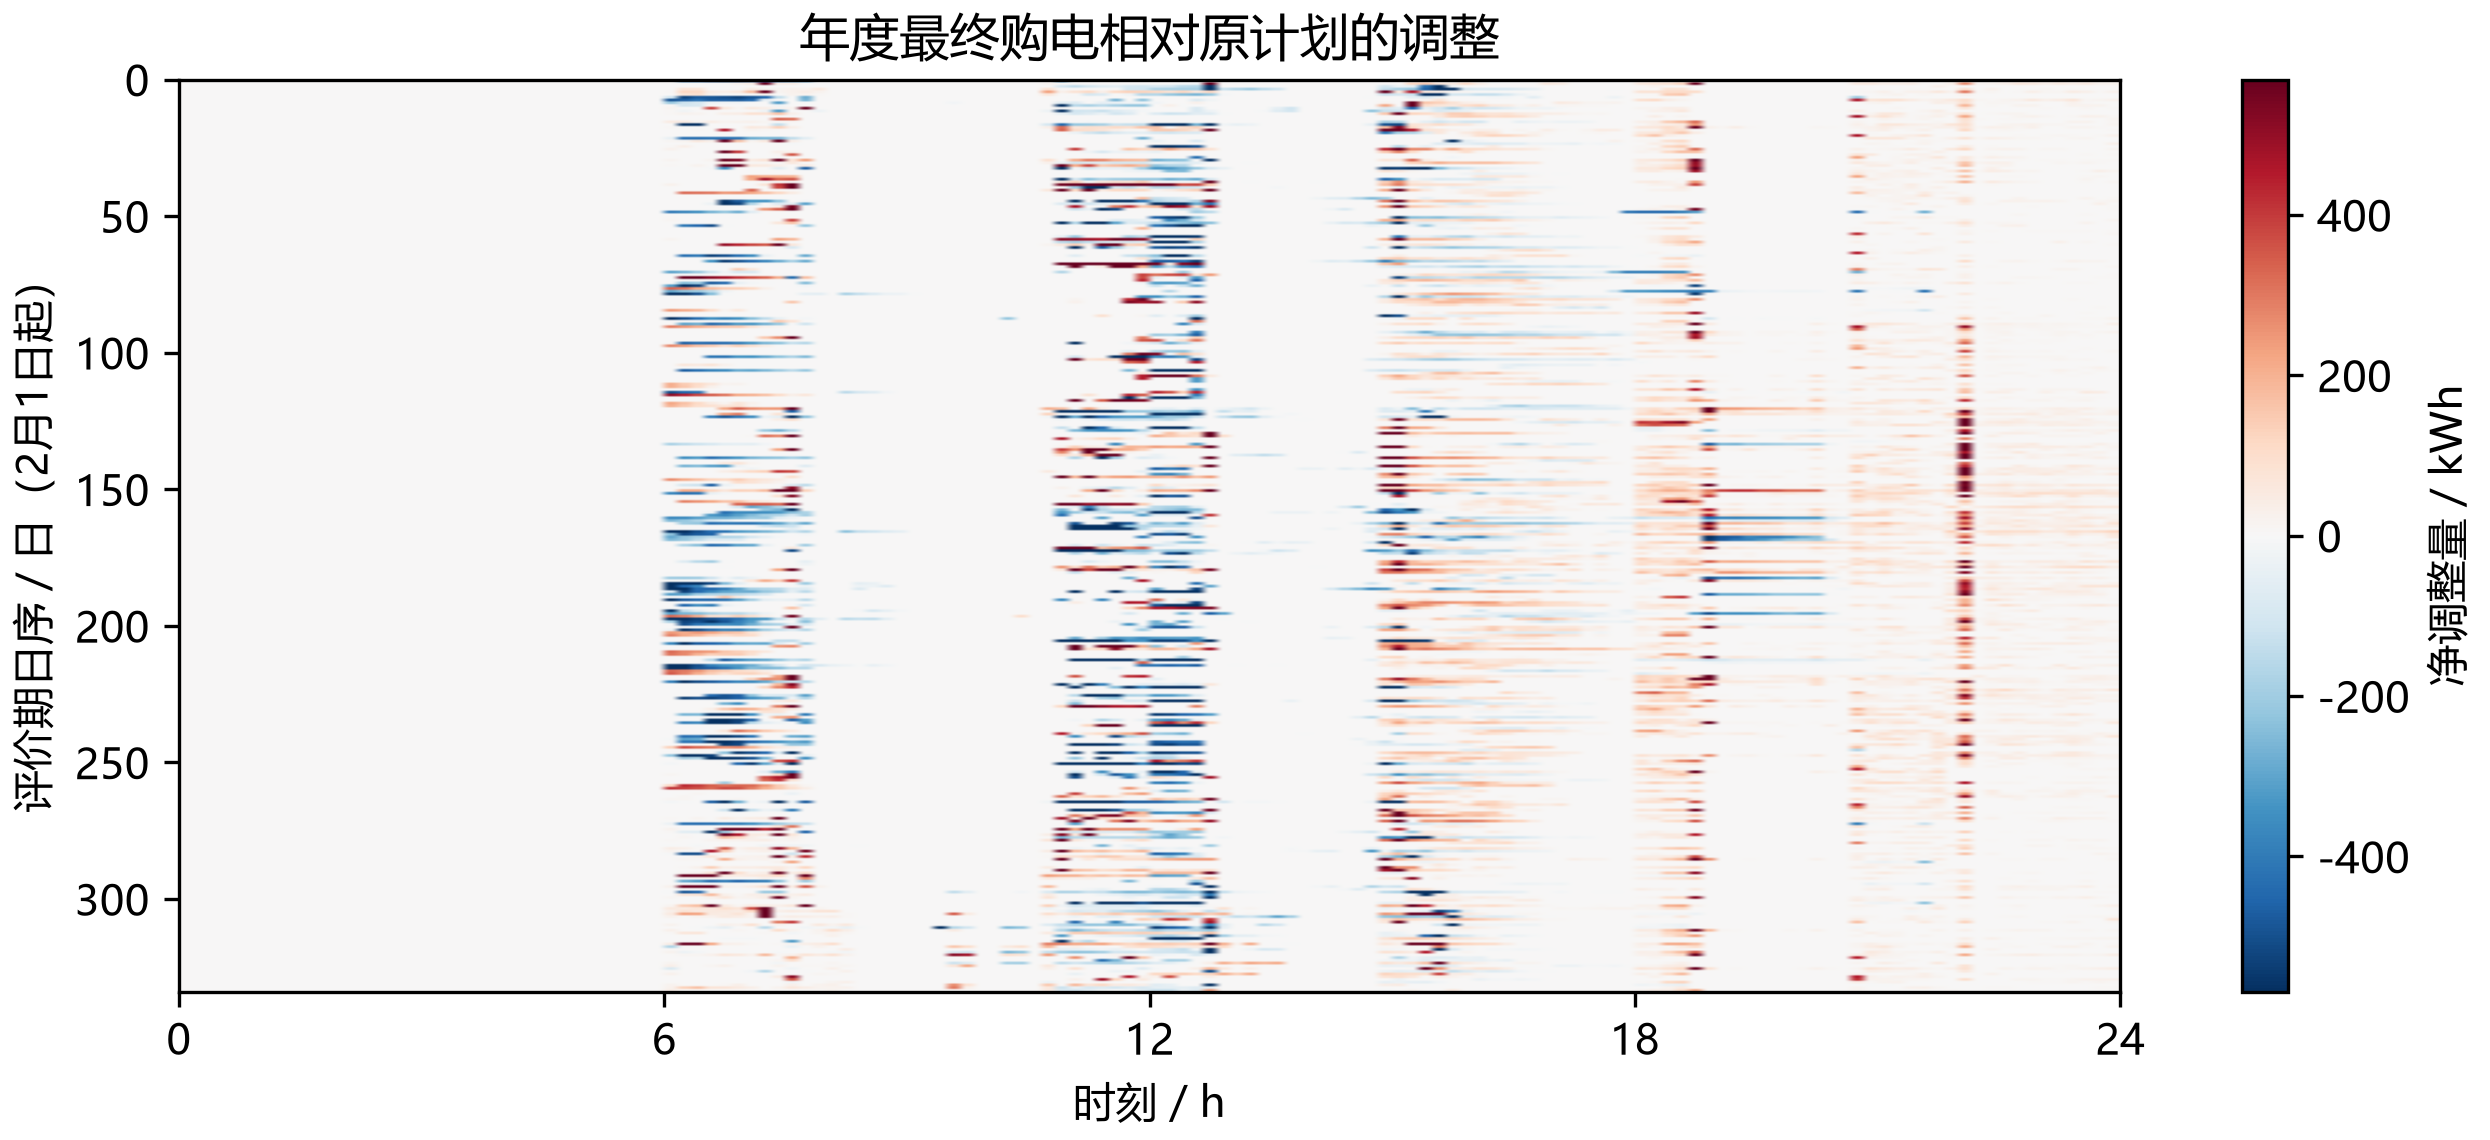
\includegraphics[width=.96\textwidth]{q3_run/paper/q3_adjustment.png}
\caption{年度购电调整时序分布}\label{fig:q3-heat}
\parbox{.94\textwidth}{\footnotesize 图注：暖色表示上调、冷色表示退款下调，色限取绝对调整量的百分之九十九分位，极值仅作显示截断。}
\end{figure}
完整334日结果保存为\texttt{q3\_run/result3.xlsx}，十分钟原始轨迹见\texttt{q3\_run/paper/all\_intervals.csv}。
